\documentclass[9pt]{article}\usepackage[]{graphicx}\usepackage[]{xcolor}
% maxwidth is the original width if it is less than linewidth
% otherwise use linewidth (to make sure the graphics do not exceed the margin)
\makeatletter
\def\maxwidth{ %
  \ifdim\Gin@nat@width>\linewidth
    \linewidth
  \else
    \Gin@nat@width
  \fi
}
\makeatother

\definecolor{fgcolor}{rgb}{0.345, 0.345, 0.345}
\newcommand{\hlnum}[1]{\textcolor[rgb]{0.686,0.059,0.569}{#1}}%
\newcommand{\hlstr}[1]{\textcolor[rgb]{0.192,0.494,0.8}{#1}}%
\newcommand{\hlcom}[1]{\textcolor[rgb]{0.678,0.584,0.686}{\textit{#1}}}%
\newcommand{\hlopt}[1]{\textcolor[rgb]{0,0,0}{#1}}%
\newcommand{\hlstd}[1]{\textcolor[rgb]{0.345,0.345,0.345}{#1}}%
\newcommand{\hlkwa}[1]{\textcolor[rgb]{0.161,0.373,0.58}{\textbf{#1}}}%
\newcommand{\hlkwb}[1]{\textcolor[rgb]{0.69,0.353,0.396}{#1}}%
\newcommand{\hlkwc}[1]{\textcolor[rgb]{0.333,0.667,0.333}{#1}}%
\newcommand{\hlkwd}[1]{\textcolor[rgb]{0.737,0.353,0.396}{\textbf{#1}}}%
\let\hlipl\hlkwb

\usepackage{framed}
\makeatletter
\newenvironment{kframe}{%
 \def\at@end@of@kframe{}%
 \ifinner\ifhmode%
  \def\at@end@of@kframe{\end{minipage}}%
  \begin{minipage}{\columnwidth}%
 \fi\fi%
 \def\FrameCommand##1{\hskip\@totalleftmargin \hskip-\fboxsep
 \colorbox{shadecolor}{##1}\hskip-\fboxsep
     % There is no \\@totalrightmargin, so:
     \hskip-\linewidth \hskip-\@totalleftmargin \hskip\columnwidth}%
 \MakeFramed {\advance\hsize-\width
   \@totalleftmargin\z@ \linewidth\hsize
   \@setminipage}}%
 {\par\unskip\endMakeFramed%
 \at@end@of@kframe}
\makeatother

\definecolor{shadecolor}{rgb}{.97, .97, .97}
\definecolor{messagecolor}{rgb}{0, 0, 0}
\definecolor{warningcolor}{rgb}{1, 0, 1}
\definecolor{errorcolor}{rgb}{1, 0, 0}
\newenvironment{knitrout}{}{} % an empty environment to be redefined in TeX

\usepackage{alltt}
\usepackage{multicol}
\usepackage{amssymb,mathrsfs,graphicx}
\usepackage{enumerate}
\usepackage{amsthm}
\usepackage{lscape}
\usepackage{pdfpages}
\theoremstyle{definition}
\newtheorem{definition}{Definition}[section]

\theoremstyle{remark}
\newtheorem{remark}{Remark}

\usepackage[colorlinks=true,linkcolor={blue},citecolor={blue},urlcolor={blue}]{hyperref}
\usepackage{longtable,ctable}
\usepackage{amsmath}
\usepackage{amssymb}
\usepackage{amsfonts}
\usepackage{multirow}
\usepackage{graphicx}
\usepackage{booktabs}
\usepackage{amsmath}
\usepackage{graphicx}
\usepackage{mathptmx}
\usepackage{natbib}
\usepackage{setspace}

\usepackage[utf8]{inputenc}
\usepackage{pgf}

\usepackage{algorithm}
\usepackage{algpseudocode}
\usepackage{enumerate}
\usepackage{threeparttable}


\newcommand{\R}{R}
\newcommand{\gbsg}{gbsg}

\def\FsNg{\hbox{FS}(M_{g})}

\def\hhat{\hat\theta(\hat{H})}
\def\hchat{\hat\theta(\hat{H}^{c})}
\def\hknow{\hat\theta(H)}
\def\hcknow{\hat\theta(H^{c})}
\def\hplim{\theta^{\dagger}(H)}
\def\hcplim{\theta^{\dagger}(H^{c})}


\newcommand{\indep}{\perp \!\!\! \perp}

\textheight=9.25in \textwidth=6.0in 
\topmargin=0in
\evensidemargin=0in \oddsidemargin=0in
\IfFileExists{upquote.sty}{\usepackage{upquote}}{}
\begin{document}

\raggedbottom


\begin{knitrout}
\definecolor{shadecolor}{rgb}{0.969, 0.969, 0.969}\color{fgcolor}\begin{kframe}
\begin{alltt}
\hlstd{opts_chunk}\hlopt{$}\hlkwd{set} \hlstd{(}\hlkwc{warning} \hlstd{=} \hlnum{FALSE}\hlstd{,} \hlkwc{message} \hlstd{=} \hlnum{FALSE}\hlstd{,} \hlkwc{tidy}\hlstd{=}\hlnum{TRUE}\hlstd{,} \hlkwc{echo}\hlstd{=}\hlnum{TRUE}\hlstd{)}
\hlkwd{options}\hlstd{(}\hlkwc{warn} \hlstd{=} \hlopt{-}\hlnum{1}\hlstd{)}

\hlkwd{rm}\hlstd{(}\hlkwc{list}\hlstd{=}\hlkwd{ls}\hlstd{())}

\hlkwd{library}\hlstd{(survival)}
\hlkwd{library}\hlstd{(knitr)}
\hlkwd{library}\hlstd{(kableExtra)}

\hlkwd{library}\hlstd{(glmnet)}
\end{alltt}


{\ttfamily\noindent\itshape\color{messagecolor}{\#\# Loading required package: Matrix}}

{\ttfamily\noindent\itshape\color{messagecolor}{\#\# Loaded glmnet 4.1-7}}\begin{alltt}
\hlkwd{library}\hlstd{(ggplot2)}

\hlcom{# Following loaded in "forest_search_v0.R"}
\hlkwd{suppressMessages}\hlstd{(}\hlkwd{library}\hlstd{(randomForest))}
\hlcom{#library(SPlit)}

\hlkwd{library}\hlstd{(grf)}
\hlkwd{library}\hlstd{(policytree)}
\hlkwd{library}\hlstd{(DiagrammeR)}

\hlcom{#library(cowplot)}

\hlkwd{library}\hlstd{(data.table)}
\hlkwd{library}\hlstd{(plyr)}
\hlkwd{library}\hlstd{(aVirtualTwins)}
\hlcom{# Not sure formatR is needed?}
\hlcom{#library(formatR)}
\hlkwd{suppressMessages}\hlstd{(}\hlkwd{library}\hlstd{(gridExtra))}

\hlkwd{library}\hlstd{(speff2trial)}
\end{alltt}


{\ttfamily\noindent\itshape\color{messagecolor}{\#\# Loading required package: leaps}}\begin{alltt}
\hlcom{# Location where code is stored}
\hlstd{codepath}\hlkwb{<-}\hlkwd{c}\hlstd{(}\hlstr{"/Users/larryleon/Documents/GitHub/forestSearch/R/"}\hlstd{)}
\hlkwd{source}\hlstd{(}\hlkwd{paste0}\hlstd{(codepath,}\hlstr{"source_forestsearch_v0.R"}\hlstd{))}
\hlkwd{source_fs_functions}\hlstd{(}\hlkwc{file_loc}\hlstd{=codepath)}

\hlstd{save_output}\hlkwb{<-}\hlnum{TRUE}
\end{alltt}
\end{kframe}
\end{knitrout}


\begin{knitrout}
\definecolor{shadecolor}{rgb}{0.969, 0.969, 0.969}\color{fgcolor}\begin{kframe}
\begin{alltt}
\hlcom{# NOTE: ZDV+DDI = arm 1, DDI = arm 3}
\hlstd{t.start.all} \hlkwb{<-} \hlkwd{proc.time}\hlstd{()[}\hlnum{3}\hlstd{]}
\hlcom{# GRF analysis To guide selection of binary cutpoints}
\hlstd{df.analysis} \hlkwb{<-} \hlkwd{subset}\hlstd{(ACTG175, arms} \hlopt \hlkwd{c}\hlstd{(}\hlnum{1}\hlstd{,} \hlnum{3}\hlstd{))}
\hlstd{df.analysis} \hlkwb{<-} \hlkwd{within}\hlstd{(df.analysis, \{}
    \hlstd{id} \hlkwb{<-} \hlkwd{as.numeric}\hlstd{(}\hlkwd{c}\hlstd{(}\hlnum{1}\hlopt{:}\hlkwd{nrow}\hlstd{(df.analysis)))}
    \hlstd{time_days} \hlkwb{<-} \hlstd{days}
    \hlstd{treat} \hlkwb{<-} \hlkwd{ifelse}\hlstd{(arms} \hlopt{==} \hlnum{1}\hlstd{,} \hlnum{1}\hlstd{,} \hlnum{0}\hlstd{)}
\hlstd{\})}

\hlcom{# plot(survfit(Surv(time_days,cens)~treat,data=df.analysis))}
\hlkwd{coxph}\hlstd{(}\hlkwd{Surv}\hlstd{(time_days, cens)} \hlopt{~} \hlstd{treat,} \hlkwc{data} \hlstd{= df.analysis)}
\end{alltt}
\begin{verbatim}
## Call:
## coxph(formula = Surv(time_days, cens) ~ treat, data = df.analysis)
## 
##          coef exp(coef) se(coef)      z     p
## treat -0.1751    0.8394   0.1324 -1.323 0.186
## 
## Likelihood ratio test=1.76  on 1 df, p=0.1849
## n= 1083, number of events= 231
\end{verbatim}
\begin{alltt}
\hlstd{confounders.name} \hlkwb{<-} \hlkwd{c}\hlstd{(}\hlstr{"age"}\hlstd{,} \hlstr{"wtkg"}\hlstd{,} \hlstr{"karnof"}\hlstd{,} \hlstr{"cd40"}\hlstd{,} \hlstr{"cd80"}\hlstd{,} \hlstr{"hemo"}\hlstd{,} \hlstr{"homo"}\hlstd{,} \hlstr{"drugs"}\hlstd{,}
    \hlstr{"race"}\hlstd{,} \hlstr{"gender"}\hlstd{,} \hlstr{"oprior"}\hlstd{,} \hlstr{"symptom"}\hlstd{)}
\hlstd{outcome.name} \hlkwb{<-} \hlkwd{c}\hlstd{(}\hlstr{"time_days"}\hlstd{)}
\hlstd{event.name} \hlkwb{<-} \hlkwd{c}\hlstd{(}\hlstr{"cens"}\hlstd{)}
\hlstd{id.name} \hlkwb{<-} \hlkwd{c}\hlstd{(}\hlstr{"id"}\hlstd{)}
\hlstd{treat.name} \hlkwb{<-} \hlkwd{c}\hlstd{(}\hlstr{"treat"}\hlstd{)}

\hlstd{n.min} \hlkwb{<-} \hlnum{60}
\hlstd{dmin.grf} \hlkwb{<-} \hlnum{12}
\hlstd{frac.tau} \hlkwb{<-} \hlnum{0.8}
\end{alltt}
\end{kframe}
\end{knitrout}


\begin{knitrout}
\definecolor{shadecolor}{rgb}{0.969, 0.969, 0.969}\color{fgcolor}\begin{kframe}
\begin{alltt}
\hlstd{grf.est} \hlkwb{<-} \hlkwd{grf.subg.harm.survival}\hlstd{(}\hlkwc{data} \hlstd{= df.analysis,} \hlkwc{confounders.name} \hlstd{= confounders.name,}
    \hlkwc{outcome.name} \hlstd{= outcome.name,} \hlkwc{event.name} \hlstd{= event.name,} \hlkwc{id.name} \hlstd{= id.name,} \hlkwc{treat.name} \hlstd{= treat.name,}
    \hlkwc{n.min} \hlstd{= n.min,} \hlkwc{dmin.grf} \hlstd{= dmin.grf,} \hlkwc{frac.tau} \hlstd{= frac.tau,} \hlkwc{details} \hlstd{=} \hlnum{TRUE}\hlstd{)}
\end{alltt}
\begin{verbatim}
## tau= 816.8 
##    leaf.node control.mean control.size control.se treated.mean treated.size
## 1          2   -24.449349   854.000000   9.828508    24.449349   854.000000
## 2          3    17.980260   229.000000  15.140988   -17.980260   229.000000
## 3          4    33.884718   147.000000  21.926236   -33.884718   147.000000
## 4          5   -49.732432   381.000000  14.216063    49.732432   381.000000
## 5          6    63.414171   100.000000  26.973648   -63.414171   100.000000
## 6          7   -20.080612   455.000000  12.913237    20.080612   455.000000
## 31        10    87.756387    70.000000  43.085562   -87.756387    70.000000
## 41        11   -58.661792   224.000000  25.870745    58.661792   224.000000
## 51        12    53.110701   100.000000  20.113294   -53.110701   100.000000
## 61        13   -37.973121   449.000000   9.850072    37.973121   449.000000
## 8         15    30.571549   164.000000  12.832862   -30.571549   164.000000
##    treated.se       diff depth
## 1    9.828508  -48.89870     1
## 2   15.140988   35.96052     1
## 3   21.926236   67.76944     2
## 4   14.216063  -99.46486     2
## 5   26.973648  126.82834     2
## 6   12.913237  -40.16122     2
## 31  43.085562  175.51277     3
## 41  25.870745 -117.32358     3
## 51  20.113294  106.22140     3
## 61   9.850072  -75.94624     3
## 8   12.832862   61.14310     3
##    leaf.node control.mean control.size control.se treated.mean treated.size
## 31        10     87.75639     70.00000   43.08556    -87.75639     70.00000
##    treated.se     diff depth
## 31   43.08556 175.5128     3
\end{verbatim}
\begin{alltt}
\hlkwd{cat}\hlstd{(}\hlstr{"Truncation point for RMST:"}\hlstd{,} \hlkwd{c}\hlstd{(grf.est}\hlopt{$}\hlstd{tau.rmst),} \hlstr{"\textbackslash{}n"}\hlstd{)}
\end{alltt}
\begin{verbatim}
## Truncation point for RMST: 816.8
\end{verbatim}
\begin{alltt}
\hlcom{# Plot manually}

\hlcom{# plot(grf.est$tree)}

\hlcom{# plot(grf.est$tree1)}

\hlcom{# plot(grf.est$tree2)}

\hlcom{# plot(grf.est$tree3)}

\hlstd{df0.grf} \hlkwb{<-} \hlkwd{subset}\hlstd{(grf.est}\hlopt{$}\hlstd{data, treat.recommend} \hlopt{==} \hlnum{0}\hlstd{)}
\hlstd{df1.grf} \hlkwb{<-} \hlkwd{subset}\hlstd{(grf.est}\hlopt{$}\hlstd{data, treat.recommend} \hlopt{==} \hlnum{1}\hlstd{)}

\hlcom{# Terminal leaf corresponding to selected SG}
\hlkwd{cat}\hlstd{(}\hlstr{"Terminal leaf:"}\hlstd{,} \hlkwd{c}\hlstd{(grf.est}\hlopt{$}\hlstd{sg.harm.id),} \hlstr{"\textbackslash{}n"}\hlstd{)}
\end{alltt}
\begin{verbatim}
## Terminal leaf: age <= 29
\end{verbatim}
\begin{alltt}
\hlcom{# action=1 --> recommend control}

\hlcom{# Manually identify the subgroup looking at tree and terminal leaf}
\hlkwd{print}\hlstd{(}\hlkwd{dim}\hlstd{(df0.grf))}
\end{alltt}
\begin{verbatim}
## [1] 70 34
\end{verbatim}
\begin{alltt}
\hlstd{check} \hlkwb{<-} \hlkwd{subset}\hlstd{(df.analysis, cd40} \hlopt{<=} \hlnum{273} \hlopt{&} \hlstd{karnof} \hlopt{>} \hlnum{80} \hlopt{&} \hlstd{age} \hlopt{<=} \hlnum{29}\hlstd{)}
\hlkwd{print}\hlstd{(}\hlkwd{dim}\hlstd{(check))}
\end{alltt}
\begin{verbatim}
## [1] 70 29
\end{verbatim}
\begin{alltt}
\hlcom{# plot(survfit(Surv(time_days,cens)~treat,data=df.analysis))}
\hlcom{# coxph(Surv(time_days,cens)~treat,data=df.analysis)}

\hlkwa{if} \hlstd{(save_output)} \hlkwd{save}\hlstd{(grf.est,} \hlkwc{file} \hlstd{=} \hlstr{"output/grf_actg_Arms_1vs3_final.Rdata"}\hlstd{)}
\end{alltt}
\end{kframe}
\end{knitrout}

%\begin{figure}[h]
%\includegraphics[width=\textwidth, height=6in]{actg_2v3_tree.png}
%\caption{GRF tree corresponding to estimated subgroup.}
%\label{fig:grftree}
%\end{figure}

%\begin{figure}[h]
%\includegraphics[width=\textwidth, height=6in]{actg_2v3_tree2.png}
%\caption{GRF depth=2 tree.}
%\label{fig:grftree2}
%\end{figure}

\begin{figure}[h!]
\begin{center}
\begin{knitrout}
\definecolor{shadecolor}{rgb}{0.969, 0.969, 0.969}\color{fgcolor}\begin{kframe}
\begin{alltt}
\hlkwd{par}\hlstd{(}\hlkwc{mfrow} \hlstd{=} \hlkwd{c}\hlstd{(}\hlnum{1}\hlstd{,} \hlnum{2}\hlstd{))}
\hlkwd{plot.subgroup}\hlstd{(}\hlkwc{sub1} \hlstd{= df0.grf,} \hlkwc{sub1C} \hlstd{= df1.grf,} \hlkwc{tte.name} \hlstd{=} \hlstr{"time_days"}\hlstd{,} \hlkwc{event.name} \hlstd{=} \hlstr{"cens"}\hlstd{,}
    \hlkwc{treat.name} \hlstd{=} \hlstr{"treat"}\hlstd{,} \hlkwc{fix.rows} \hlstd{=} \hlnum{FALSE}\hlstd{,} \hlkwc{byrisk} \hlstd{=} \hlnum{200}\hlstd{,} \hlkwc{show.med} \hlstd{=} \hlnum{FALSE}\hlstd{,} \hlkwc{ymin} \hlstd{=} \hlnum{0.4}\hlstd{)}
\end{alltt}
\end{kframe}
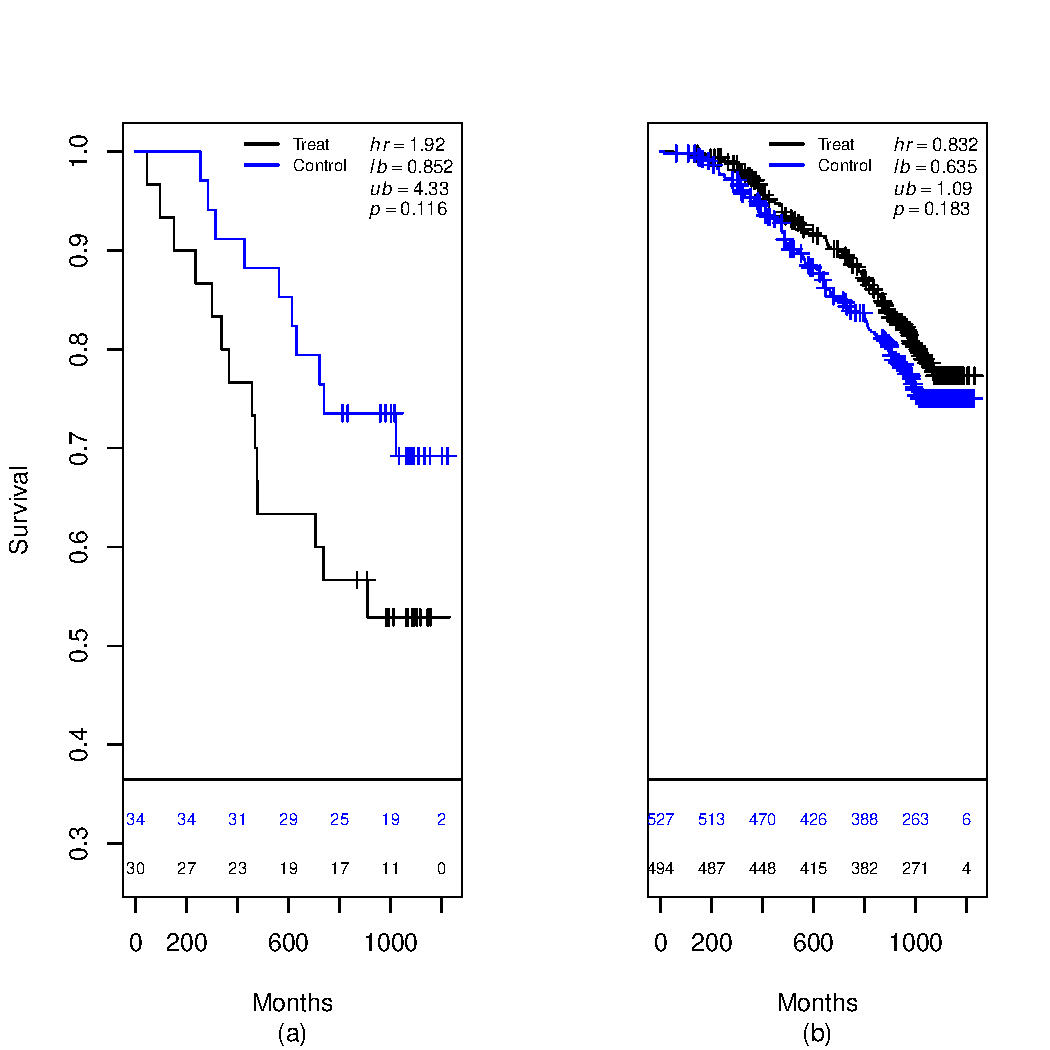
\includegraphics[width=400px,height=400px]{figure/grf_sg-1} 
\end{knitrout}
\end{center}
\end{figure}


\begin{knitrout}
\definecolor{shadecolor}{rgb}{0.969, 0.969, 0.969}\color{fgcolor}\begin{kframe}
\begin{alltt}
\hlcom{# Stored results load('output/grf_actg_Arms_1vs3_final.Rdata')}

\hlkwd{cat}\hlstd{(}\hlstr{"GRF variables in selected tree"}\hlstd{,} \hlstr{"\textbackslash{}n"}\hlstd{)}
\end{alltt}
\begin{verbatim}
## GRF variables in selected tree
\end{verbatim}
\begin{alltt}
\hlkwd{print}\hlstd{(grf.est}\hlopt{$}\hlstd{tree.names)}
\end{alltt}
\begin{verbatim}
## [1] "cd40"   "karnof" "wtkg"   "age"
\end{verbatim}
\begin{alltt}
\hlkwd{cat}\hlstd{(}\hlstr{"GRF cuts wrt selected tree:"}\hlstd{,} \hlstr{"\textbackslash{}n"}\hlstd{)}
\end{alltt}
\begin{verbatim}
## GRF cuts wrt selected tree:
\end{verbatim}
\begin{alltt}
\hlkwd{print}\hlstd{(grf.est}\hlopt{$}\hlstd{tree.cuts)}
\end{alltt}
\begin{verbatim}
## [1] "cd40 <= 273"  "karnof <= 80" "wtkg <= 81.7" "age <= 34"    "age <= 29"   
## [6] "cd40 <= 311"  "cd40 <= 321"
\end{verbatim}
\begin{alltt}
\hlcom{# Reduce dimension via Cox lasso}

\hlstd{xx} \hlkwb{<-} \hlkwd{as.matrix}\hlstd{(df.analysis[, confounders.name])}
\hlstd{yy} \hlkwb{<-} \hlkwd{as.matrix}\hlstd{(df.analysis[,} \hlkwd{c}\hlstd{(}\hlstr{"time_days"}\hlstd{,} \hlstr{"cens"}\hlstd{)])}
\hlkwd{colnames}\hlstd{(yy)} \hlkwb{<-} \hlkwd{c}\hlstd{(}\hlstr{"time"}\hlstd{,} \hlstr{"status"}\hlstd{)}

\hlstd{cvfit} \hlkwb{<-} \hlkwd{cv.glmnet}\hlstd{(xx, yy,} \hlkwc{family} \hlstd{=} \hlstr{"cox"}\hlstd{)}  \hlcom{#first do 10-fold cross-validation to select lambda}

\hlstd{m} \hlkwb{<-} \hlkwd{glmnet}\hlstd{(xx, yy,} \hlkwc{family} \hlstd{=} \hlstr{"cox"}\hlstd{,} \hlkwc{lambda} \hlstd{= cvfit}\hlopt{$}\hlstd{lambda.min)}  \hlcom{#plugin the optimal lambda}

\hlstd{conflasso.name} \hlkwb{<-} \hlstd{confounders.name[}\hlkwd{which}\hlstd{(m}\hlopt{$}\hlstd{beta} \hlopt{!=} \hlnum{0}\hlstd{)]}

\hlkwd{cat}\hlstd{(}\hlstr{"Cox-LASSO selected:"}\hlstd{,} \hlkwd{c}\hlstd{(conflasso.name),} \hlstr{"\textbackslash{}n"}\hlstd{)}
\end{alltt}
\begin{verbatim}
## Cox-LASSO selected: wtkg karnof cd40 cd80 homo race symptom
\end{verbatim}
\begin{alltt}
\hlkwd{cat}\hlstd{(}\hlstr{"GRF cuts wrt selected tree:"}\hlstd{,} \hlstr{"\textbackslash{}n"}\hlstd{)}
\end{alltt}
\begin{verbatim}
## GRF cuts wrt selected tree:
\end{verbatim}
\begin{alltt}
\hlkwd{print}\hlstd{(grf.est}\hlopt{$}\hlstd{tree.cuts)}
\end{alltt}
\begin{verbatim}
## [1] "cd40 <= 273"  "karnof <= 80" "wtkg <= 81.7" "age <= 34"    "age <= 29"   
## [6] "cd40 <= 311"  "cd40 <= 321"
\end{verbatim}
\begin{alltt}
\hlcom{#'cd40 <= 273'  'karnof <= 80' 'wtkg <= 81.7' 'age <= 34'    'age <= 29'    'cd40 <= 311'  'cd40 <= 321' }

\hlcom{# Cox-LASSO selected: wtkg karnof cd40 cd80 hemo homo race symptom}

\hlcom{# Considering continuous factors per GRF cuts Only considering hemo, homo,}
\hlcom{# race, and symptom per lasso}
\hlstd{df.analysis} \hlkwb{<-} \hlkwd{within}\hlstd{(df.analysis, \{}
    \hlcom{# Age at 29 and 34}
    \hlstd{z1a} \hlkwb{<-} \hlkwd{ifelse}\hlstd{(age} \hlopt{<=} \hlnum{29}\hlstd{,} \hlnum{1}\hlstd{,} \hlnum{0}\hlstd{)}
    \hlstd{z1b} \hlkwb{<-} \hlkwd{ifelse}\hlstd{(age} \hlopt{<=} \hlnum{34}\hlstd{,} \hlnum{1}\hlstd{,} \hlnum{0}\hlstd{)}
    \hlcom{# Wtkg 81.7}
    \hlstd{z2} \hlkwb{<-} \hlkwd{ifelse}\hlstd{(wtkg} \hlopt{<=} \hlnum{82}\hlstd{,} \hlnum{1}\hlstd{,} \hlnum{0}\hlstd{)}
    \hlcom{# Karnof 80}
    \hlstd{z3} \hlkwb{<-} \hlkwd{ifelse}\hlstd{(karnof} \hlopt{<=} \hlnum{80}\hlstd{,} \hlnum{1}\hlstd{,} \hlnum{0}\hlstd{)}
    \hlcom{# cd80 ---> median}
    \hlstd{z4} \hlkwb{<-} \hlkwd{ifelse}\hlstd{(cd80} \hlopt{<=} \hlkwd{median}\hlstd{(cd80),} \hlnum{1}\hlstd{,} \hlnum{0}\hlstd{)}
    \hlcom{# cd40 273, 311, 321}
    \hlstd{z5a} \hlkwb{<-} \hlkwd{ifelse}\hlstd{(cd40} \hlopt{<=} \hlnum{273}\hlstd{,} \hlnum{1}\hlstd{,} \hlnum{0}\hlstd{)}
    \hlstd{z5b} \hlkwb{<-} \hlkwd{ifelse}\hlstd{(cd40} \hlopt{<=} \hlnum{311}\hlstd{,} \hlnum{1}\hlstd{,} \hlnum{0}\hlstd{)}
    \hlstd{z5c} \hlkwb{<-} \hlkwd{ifelse}\hlstd{(cd40} \hlopt{<=} \hlnum{321}\hlstd{,} \hlnum{1}\hlstd{,} \hlnum{0}\hlstd{)}
    \hlstd{z6} \hlkwb{<-} \hlstd{hemo}
    \hlstd{z7} \hlkwb{<-} \hlstd{homo}
    \hlcom{# z8<-drugs}
    \hlstd{z9} \hlkwb{<-} \hlstd{race}
    \hlcom{# z10<-gender z11<-oprior}
    \hlstd{z12} \hlkwb{<-} \hlstd{symptom}
    \hlcom{# Convert to factors}
    \hlstd{v1a} \hlkwb{<-} \hlkwd{as.factor}\hlstd{(z1a)}
    \hlstd{v1b} \hlkwb{<-} \hlkwd{as.factor}\hlstd{(z1b)}
    \hlstd{v2} \hlkwb{<-} \hlkwd{as.factor}\hlstd{(z2)}
    \hlstd{v3} \hlkwb{<-} \hlkwd{as.factor}\hlstd{(z3)}
    \hlstd{v4} \hlkwb{<-} \hlkwd{as.factor}\hlstd{(z4)}
    \hlstd{v5a} \hlkwb{<-} \hlkwd{as.factor}\hlstd{(z5a)}
    \hlstd{v5b} \hlkwb{<-} \hlkwd{as.factor}\hlstd{(z5b)}
    \hlstd{v5c} \hlkwb{<-} \hlkwd{as.factor}\hlstd{(z5c)}
    \hlstd{v6} \hlkwb{<-} \hlkwd{as.factor}\hlstd{(z6)}
    \hlstd{v7} \hlkwb{<-} \hlkwd{as.factor}\hlstd{(z7)}
    \hlstd{v8} \hlkwb{<-} \hlkwd{as.factor}\hlstd{(z9)}
    \hlstd{v9} \hlkwb{<-} \hlkwd{as.factor}\hlstd{(z12)}
\hlstd{\})}

\hlstd{FSconfounders.name} \hlkwb{<-} \hlkwd{c}\hlstd{(}\hlstr{"v1a"}\hlstd{,} \hlstr{"v1b"}\hlstd{,} \hlstr{"v2"}\hlstd{,} \hlstr{"v3"}\hlstd{,} \hlstr{"v4"}\hlstd{,} \hlstr{"v5a"}\hlstd{,} \hlstr{"v5b"}\hlstd{,} \hlstr{"v5c"}\hlstd{,} \hlstr{"v6"}\hlstd{,}
    \hlstr{"v7"}\hlstd{,} \hlstr{"v8"}\hlstd{,} \hlstr{"v9"}\hlstd{)}

\hlstd{outcome.name} \hlkwb{<-} \hlkwd{c}\hlstd{(}\hlstr{"time_days"}\hlstd{)}
\hlstd{event.name} \hlkwb{<-} \hlkwd{c}\hlstd{(}\hlstr{"cens"}\hlstd{)}
\hlstd{id.name} \hlkwb{<-} \hlkwd{c}\hlstd{(}\hlstr{"id"}\hlstd{)}
\hlstd{treat.name} \hlkwb{<-} \hlkwd{c}\hlstd{(}\hlstr{"treat"}\hlstd{)}

\hlstd{df.confounders} \hlkwb{<-} \hlstd{df.analysis[, FSconfounders.name]}
\hlstd{df.confounders} \hlkwb{<-} \hlkwd{dummy}\hlstd{(df.confounders)}

\hlstd{hr.threshold} \hlkwb{<-} \hlnum{1.5}  \hlcom{# Initital candidates }
\hlstd{hr.consistency} \hlkwb{<-} \hlnum{1.25}  \hlcom{# Candidates for many splits}

\hlstd{pconsistency.threshold} \hlkwb{<-} \hlnum{0.9}
\hlstd{maxk} \hlkwb{<-} \hlnum{4}
\hlcom{# maxk is max # of covariates in combination Since we want to allow generation}
\hlcom{# of intervals for single covariate allowing for 4 can yield v1, v2 (say), and}
\hlcom{# v3,v4 with v3 and v4 generating intervals for a single covariate}

\hlcom{# Limit timing for forestsearch}
\hlstd{max.minutes} \hlkwb{<-} \hlnum{60}
\hlstd{nmin.fs} \hlkwb{<-} \hlnum{60}
\hlcom{# stop.threshold<-0.60 # If any sg meets this, then choose this (stop here);}
\hlstd{m1.threshold} \hlkwb{<-} \hlnum{Inf}  \hlcom{# Turning this off (Default)}
\hlstd{stop.threshold} \hlkwb{<-} \hlnum{1}
\hlcom{# =1 will run through all sg's meeting HR criteria pconsistency.threshold<-0.70}
\hlcom{# # Minimum threshold (will choose max among subgroups satisfying)}
\hlstd{fs.splits} \hlkwb{<-} \hlnum{1000}  \hlcom{# How many times to split for consistency}
\hlcom{# vi is % factor is selected in cross-validation --> higher more important Set}
\hlcom{# liberal here, since LASSO used for selection; VI (variable importance per}
\hlcom{# GRF) used for sorting}
\hlstd{vi.grf.min} \hlkwb{<-} \hlnum{0.1}
\hlcom{# Null, turns off grf screening Set to 5 for this heavily censored data}
\hlstd{d.min} \hlkwb{<-} \hlnum{5}  \hlcom{# Min number of events for both arms (d0.min=d1.min=d.min)}
\hlcom{# default=5}

\hlstd{sg_focus} \hlkwb{<-} \hlstr{"hr"}
\hlstd{split_method} \hlkwb{<-} \hlstr{"Random"}
\hlstd{pstop_futile} \hlkwb{<-} \hlnum{0.3}
\hlcom{# Stops the consistency evaluation after first subgroup with consistency below}
\hlcom{# pstop_futile With idea that since SG's are sorted by hazard ratio estimates,}
\hlcom{# once consistency is below pstop_futile it seems unlikely that SG's with lower}
\hlcom{# hr's will reach the required consistency criterion}

\hlcom{# load('output/fs_actg_Arms_1vs3_final.Rdata') fs.est<-fs_actg_final}

\hlstd{fs.est} \hlkwb{<-} \hlkwd{forestsearch}\hlstd{(}\hlkwc{df} \hlstd{= df.analysis,} \hlkwc{confounders.name} \hlstd{= FSconfounders.name,} \hlkwc{df.predict} \hlstd{= df.analysis,}
    \hlkwc{details} \hlstd{=} \hlnum{TRUE}\hlstd{,} \hlkwc{sg_focus} \hlstd{= sg_focus,} \hlkwc{split_method} \hlstd{= split_method,} \hlkwc{pstop_futile} \hlstd{= pstop_futile,}
    \hlkwc{outcome.name} \hlstd{= outcome.name,} \hlkwc{treat.name} \hlstd{= treat.name,} \hlkwc{event.name} \hlstd{= event.name,}
    \hlkwc{id.name} \hlstd{= id.name,} \hlkwc{n.min} \hlstd{= nmin.fs,} \hlkwc{hr.threshold} \hlstd{= hr.threshold,} \hlkwc{hr.consistency} \hlstd{= hr.consistency,}
    \hlkwc{fs.splits} \hlstd{= fs.splits,} \hlkwc{stop.threshold} \hlstd{= stop.threshold,} \hlkwc{d0.min} \hlstd{= d.min,} \hlkwc{d1.min} \hlstd{= d.min,}
    \hlkwc{pconsistency.threshold} \hlstd{= pconsistency.threshold,} \hlkwc{max.minutes} \hlstd{= max.minutes,} \hlkwc{maxk} \hlstd{= maxk,}
    \hlkwc{plot.sg} \hlstd{=} \hlnum{FALSE}\hlstd{,} \hlkwc{vi.grf.min} \hlstd{= vi.grf.min)}
\end{alltt}
\begin{verbatim}
## Confounders per grf screening v1b v9 v1a v5a v7 v2 v5b v4 v8 v5c v6 v3 
## Number of possible subgroups= 16777215 
## Number of possible subgroups (in millions)= 16.77722 
## # of subgroups based on # variables > k.max and excluded 16764265 
## k.max= 4 
## Events criteria for control,exp= 5 5 
## # of subgroups with events less than criteria: control, experimental 7629 7957 
## # of subgroups meeting all criteria = 2835 
## # of subgroups fitted (Cox model estimable) = 2835 
## Minutes= 1.123433 
## Number of criteria not met for subgroup evaluation 
## crit.failure
##        0        1        2        3        4 
## 16767100      661     6674      938     1842 
## Number of subgroups meeting HR threshold 153 
## Subgroups (1st 10) meeting overall screening thresholds (HR, m1) sorted by focus: (m1,sg_focus)= Inf hr 
##     K   n  E d1  m1  m0   HR L(HR) U(HR) v1b.0 v1b.1 v9.0 v9.1 v1a.0 v1a.1
##  1: 4  91 21 16 Inf Inf 3.15  1.15  8.61     0     0    0    0     0     1
##  2: 3 105 25 17 Inf Inf 2.91  1.25  6.75     0     0    0    0     0     1
##  3: 4 105 25 17 Inf Inf 2.91  1.25  6.75     0     1    0    0     0     1
##  4: 4  79 14  9 Inf Inf 2.89  0.97  8.64     0     1    1    0     0     0
##  5: 3  90 16 10 Inf Inf 2.79  1.01  7.67     0     1    0    0     0     0
##  6: 3  64 14  9 Inf Inf 2.79  0.93  8.32     0     1    0    0     1     0
##  7: 3  72 16 11 Inf Inf 2.72  0.94  7.83     0     0    0    0     0     1
##  8: 4  72 16 11 Inf Inf 2.72  0.94  7.83     0     1    0    0     0     1
##  9: 4  66 13  8 Inf Inf 2.64  0.86  8.09     0     1    1    0     0     0
## 10: 3  70 18 12 Inf Inf 2.58  0.97  6.88     0     0    0    0     0     1
##     v5a.0 v5a.1 v7.0 v7.1 v2.0 v2.1 v5b.0 v5b.1 v4.0 v4.1 v8.0 v8.1 v5c.0 v5c.1
##  1:     0     0    0    0    0    1     0     0    0    0    0    0     0     1
##  2:     0     0    0    0    0    0     0     1    0    0    0    0     0     0
##  3:     0     0    0    0    0    0     0     1    0    0    0    0     0     0
##  4:     1     0    0    0    1    0     0     0    0    0    0    0     0     0
##  5:     1     0    0    0    1    0     0     0    0    0    0    0     0     0
##  6:     0     0    0    0    1    0     0     0    0    0    0    0     0     0
##  7:     0     0    0    0    0    0     0     1    0    0    1    0     0     0
##  8:     0     0    0    0    0    0     0     1    0    0    1    0     0     0
##  9:     0     0    0    0    1    0     0     0    0    0    1    0     0     0
## 10:     0     1    0    0    0    0     0     0    0    0    0    0     0     0
##     v6.0 v6.1 v3.0 v3.1
##  1:    0    0    1    0
##  2:    0    0    1    0
##  3:    0    0    1    0
##  4:    0    0    0    0
##  5:    0    0    0    0
##  6:    0    0    0    0
##  7:    0    0    0    0
##  8:    0    0    0    0
##  9:    0    0    0    0
## 10:    0    0    1    0
## Consistency 0.962 
## Splitting method, # of splits= Random 1000 
## Model, % Consistency Met= v1a.1 v2.1 v5c.1 v3.0 0.962 
## Consistency 0.966 
## Splitting method, # of splits= Random 1000 
## Model, % Consistency Met= v1a.1 v5b.1 v3.0 0.966 
## Consistency 0.966 
## Splitting method, # of splits= Random 1000 
## Model, % Consistency Met= v1b.1 v1a.1 v5b.1 v3.0 0.966 
## Consistency 0.665 
## Consistency 0.683 
## Consistency 0.668 
## Consistency 0.662 
## Consistency 0.662 
## Consistency 0.428 
## Consistency 0.544 
## Consistency 0.544 
## Consistency 0.624 
## Consistency 0.48 
## Consistency 0.488 
## Consistency 0.514 
## Consistency 0.514 
## Consistency 0.514 
## Consistency 0.514 
## Consistency 0.607 
## Consistency 0.384 
## Consistency 0.384 
## Consistency 0.384 
## Consistency 0.92 
## Splitting method, # of splits= Random 1000 
## Model, % Consistency Met= v1a.1 v5c.1 v3.0 0.92 
## Consistency 0.92 
## Splitting method, # of splits= Random 1000 
## Model, % Consistency Met= v1b.1 v1a.1 v5c.1 v3.0 0.92 
## Consistency 0.521 
## Consistency 0.697 
## Consistency 0.28 
## Number of subgroups meeting consistency criteria= 5 
##    p.consistency Nsg group.id m.index K   M.1   M.2   M.3  M.4
## 1:         0.962  91      135       1 4 v1a.1  v2.1 v5c.1 v3.0
## 2:         0.966 105      150       2 3 v1a.1 v5b.1  v3.0     
## 3:         0.966 105      149       3 4 v1b.1 v1a.1 v5b.1 v3.0
## 4:          0.92 113      134      23 3 v1a.1 v5c.1  v3.0     
## 5:          0.92 113      133      24 4 v1b.1 v1a.1 v5c.1 v3.0
##    p.consistency Nsg group.id m.index K   M.1   M.2   M.3  M.4
## 1:         0.966 105      150       2 3 v1a.1 v5b.1  v3.0     
## 2:         0.966 105      149       3 4 v1b.1 v1a.1 v5b.1 v3.0
## 3:         0.962  91      135       1 4 v1a.1  v2.1 v5c.1 v3.0
## 4:         0.920 113      134      23 3 v1a.1 v5c.1  v3.0     
## 5:         0.920 113      133      24 4 v1b.1 v1a.1 v5c.1 v3.0
\end{verbatim}
\begin{alltt}
\hlstd{xx} \hlkwb{<-} \hlstd{fs.est}\hlopt{$}\hlstd{find.grps}\hlopt{$}\hlstd{out.found}\hlopt{$}\hlstd{hr.subgroups}
\hlstd{covs.found} \hlkwb{<-} \hlstd{xx[,} \hlopt{-}\hlkwd{c}\hlstd{(}\hlnum{1}\hlopt{:}\hlnum{10}\hlstd{)]}
\hlstd{covs.most} \hlkwb{<-} \hlkwd{apply}\hlstd{(covs.found,} \hlnum{2}\hlstd{, sum)}
\hlstd{covs.most} \hlkwb{<-} \hlstd{covs.most[covs.most} \hlopt{>} \hlnum{0}\hlstd{]}
\hlkwd{print}\hlstd{(covs.most)}
\end{alltt}
\begin{verbatim}
## v1b.1  v9.0  v9.1 v1a.0 v1a.1 v5a.0 v5a.1  v7.0  v7.1  v2.0  v2.1 v5b.0 v5b.1 
##    86    27     3    11    50    39     9    10    11    34    28    18    40 
##  v4.0  v4.1  v8.0 v5c.0 v5c.1  v6.0  v3.0 
##    35    22    32    14    32    21    24
\end{verbatim}
\begin{alltt}
\hlkwd{print}\hlstd{(fs.est}\hlopt{$}\hlstd{grp.consistency}\hlopt{$}\hlstd{result)}
\end{alltt}
\begin{verbatim}
##    p.consistency Nsg group.id m.index K   M.1   M.2   M.3  M.4
## 1:         0.966 105      150       2 3 v1a.1 v5b.1  v3.0     
## 2:         0.966 105      149       3 4 v1b.1 v1a.1 v5b.1 v3.0
## 3:         0.962  91      135       1 4 v1a.1  v2.1 v5c.1 v3.0
## 4:         0.920 113      134      23 3 v1a.1 v5c.1  v3.0     
## 5:         0.920 113      133      24 4 v1b.1 v1a.1 v5c.1 v3.0
\end{verbatim}
\begin{alltt}
\hlstd{fs_actg_final} \hlkwb{<-} \hlstd{fs.est}

\hlstd{df0.fs} \hlkwb{<-} \hlkwd{subset}\hlstd{(fs.est}\hlopt{$}\hlstd{df.pred, treat.recommend} \hlopt{==} \hlnum{0}\hlstd{)}
\hlstd{df1.fs} \hlkwb{<-} \hlkwd{subset}\hlstd{(fs.est}\hlopt{$}\hlstd{df.pred, treat.recommend} \hlopt{==} \hlnum{1}\hlstd{)}

\hlkwa{if} \hlstd{(save_output)} \hlkwd{save}\hlstd{(fs_actg_final, df.analysis, FSconfounders.name,} \hlkwc{file} \hlstd{=} \hlstr{"output/fs_actg_Arms_1vs3_final.Rdata"}\hlstd{)}
\end{alltt}
\end{kframe}
\end{knitrout}

\begin{figure}[h!]
\begin{center}
\begin{knitrout}
\definecolor{shadecolor}{rgb}{0.969, 0.969, 0.969}\color{fgcolor}\begin{kframe}
\begin{alltt}
\hlcom{# Compare with GRF}
\hlkwd{layout}\hlstd{(}\hlkwd{matrix}\hlstd{(}\hlkwd{c}\hlstd{(}\hlnum{1}\hlstd{,} \hlnum{2}\hlstd{,} \hlnum{3}\hlstd{,} \hlnum{4}\hlstd{),} \hlnum{2}\hlstd{,} \hlnum{2}\hlstd{,} \hlkwc{byrow} \hlstd{=} \hlnum{TRUE}\hlstd{))}
\hlkwd{plot.subgroup}\hlstd{(}\hlkwc{sub1} \hlstd{= df0.grf,} \hlkwc{sub1C} \hlstd{= df1.grf,} \hlkwc{tte.name} \hlstd{=} \hlstr{"time_days"}\hlstd{,} \hlkwc{event.name} \hlstd{=} \hlstr{"cens"}\hlstd{,}
    \hlkwc{treat.name} \hlstd{=} \hlstr{"treat"}\hlstd{,} \hlkwc{fix.rows} \hlstd{=} \hlnum{FALSE}\hlstd{,} \hlkwc{byrisk} \hlstd{=} \hlnum{200}\hlstd{,} \hlkwc{show.med} \hlstd{=} \hlnum{FALSE}\hlstd{,} \hlkwc{ymin} \hlstd{=} \hlnum{0.4}\hlstd{)}
\hlkwd{plot.subgroup}\hlstd{(}\hlkwc{sub1} \hlstd{= df0.fs,} \hlkwc{sub1C} \hlstd{= df1.fs,} \hlkwc{tte.name} \hlstd{=} \hlstr{"time_days"}\hlstd{,} \hlkwc{event.name} \hlstd{=} \hlstr{"cens"}\hlstd{,}
    \hlkwc{treat.name} \hlstd{=} \hlstr{"treat"}\hlstd{,} \hlkwc{fix.rows} \hlstd{=} \hlnum{FALSE}\hlstd{,} \hlkwc{byrisk} \hlstd{=} \hlnum{200}\hlstd{,} \hlkwc{show.med} \hlstd{=} \hlnum{FALSE}\hlstd{,} \hlkwc{ymin} \hlstd{=} \hlnum{0.4}\hlstd{)}
\end{alltt}
\end{kframe}
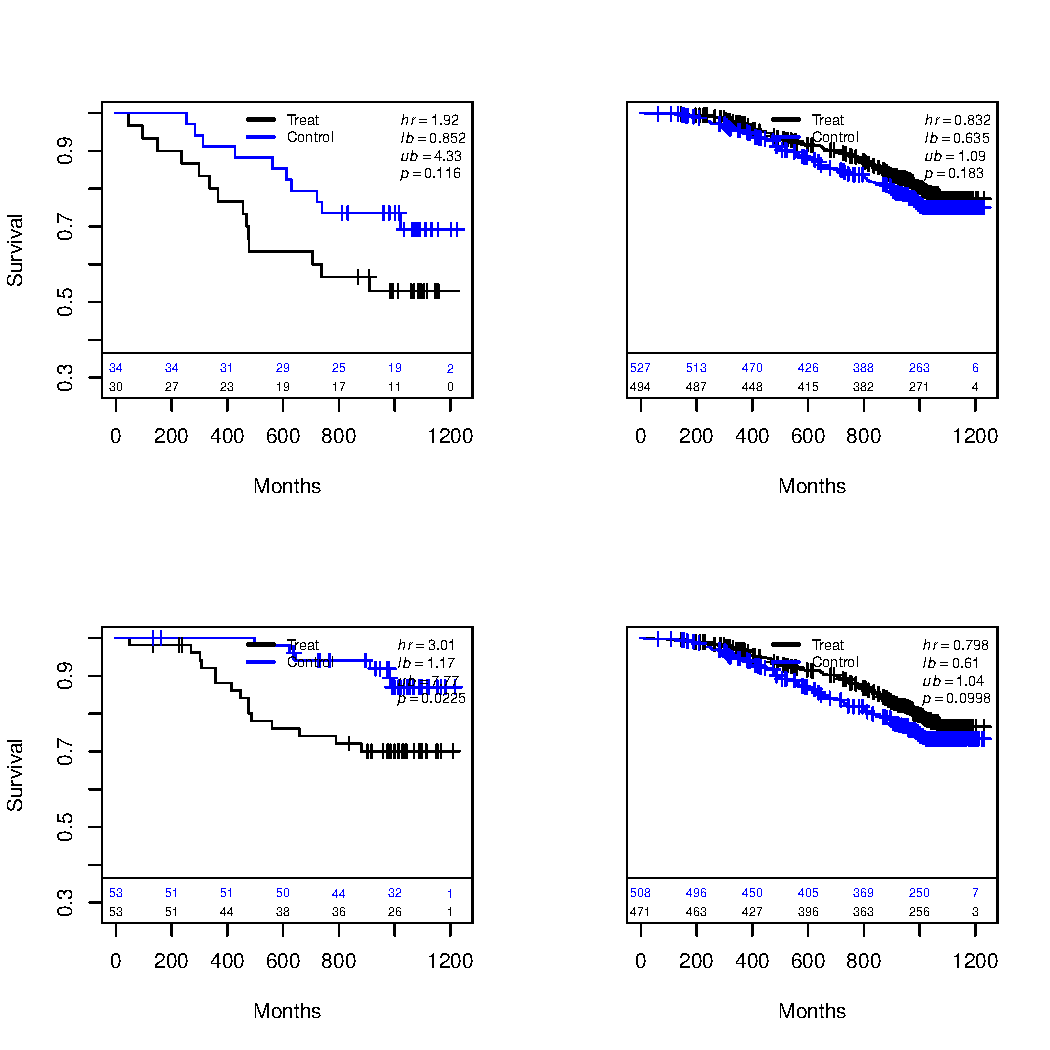
\includegraphics[width=400px,height=400px]{figure/grf-fs_sg-1} 
\end{knitrout}
\end{center}
\end{figure}


\begin{knitrout}
\definecolor{shadecolor}{rgb}{0.969, 0.969, 0.969}\color{fgcolor}\begin{kframe}
\begin{alltt}
\hlcom{# Note, the elements above will need to be re-initiated if running separate}
\hlcom{# from above E.g., outcome.names, event.name, ... hr.threshold, etc.}

\hlcom{# load('output/fs_actg_Arms_1vs3_final.Rdata') fs.est<-fs_actg_final}

\hlkwd{library}\hlstd{(doParallel)}
\hlkwd{registerDoParallel}\hlstd{(parallel}\hlopt{::}\hlkwd{detectCores}\hlstd{(}\hlkwc{logical} \hlstd{=} \hlnum{FALSE}\hlstd{))}

\hlstd{cox.formula.boot} \hlkwb{<-} \hlkwd{as.formula}\hlstd{(}\hlkwd{paste}\hlstd{(}\hlstr{"Surv(time_days,cens)~treat"}\hlstd{))}
\hlstd{est.loghr} \hlkwb{<-} \hlnum{TRUE}

\hlstd{confounders.name} \hlkwb{<-} \hlstd{FSconfounders.name}
\hlstd{stop.threshold} \hlkwb{<-} \hlnum{0.99}
\hlstd{max.minutes} \hlkwb{<-} \hlnum{6}

\hlcom{# Suggest running 50, first ... to get timing estimate}
\hlstd{NB} \hlkwb{<-} \hlnum{500}

\hlstd{df_temp} \hlkwb{<-} \hlstd{fs.est}\hlopt{$}\hlstd{df.pred[,} \hlkwd{c}\hlstd{(}\hlstr{"id"}\hlstd{,} \hlstr{"treat.recommend"}\hlstd{)]}
\hlstd{dfa} \hlkwb{<-} \hlkwd{merge}\hlstd{(df.analysis, df_temp,} \hlkwc{by} \hlstd{=} \hlstr{"id"}\hlstd{)}
\hlstd{df_boot_analysis} \hlkwb{<-} \hlstd{dfa}

\hlstd{fitH} \hlkwb{<-} \hlkwd{get_Cox_sg}\hlstd{(}\hlkwc{df_sg} \hlstd{=} \hlkwd{subset}\hlstd{(df_boot_analysis, treat.recommend} \hlopt{==} \hlnum{0}\hlstd{),} \hlkwc{cox.formula} \hlstd{= cox.formula.boot,}
    \hlkwc{est.loghr} \hlstd{= est.loghr)}
\hlstd{H_obs} \hlkwb{<-} \hlstd{fitH}\hlopt{$}\hlstd{est_obs}  \hlcom{# log(hr) scale}
\hlstd{seH_obs} \hlkwb{<-} \hlstd{fitH}\hlopt{$}\hlstd{se_obs}
\hlcom{# Hc observed estimates}
\hlstd{fitHc} \hlkwb{<-} \hlkwd{get_Cox_sg}\hlstd{(}\hlkwc{df_sg} \hlstd{=} \hlkwd{subset}\hlstd{(df_boot_analysis, treat.recommend} \hlopt{==} \hlnum{1}\hlstd{),} \hlkwc{cox.formula} \hlstd{= cox.formula.boot,}
    \hlkwc{est.loghr} \hlstd{= est.loghr)}
\hlstd{Hc_obs} \hlkwb{<-} \hlstd{fitHc}\hlopt{$}\hlstd{est_obs}
\hlstd{seHc_obs} \hlkwb{<-} \hlstd{fitHc}\hlopt{$}\hlstd{se_obs}
\hlkwd{rm}\hlstd{(}\hlstr{"fitH"}\hlstd{,} \hlstr{"fitHc"}\hlstd{)}

\hlstd{Ystar_mat} \hlkwb{<-} \hlkwd{bootYstar}\hlstd{(\{}
    \hlstd{ystar} \hlkwb{<-} \hlkwd{get_Ystar}\hlstd{(boot)}
\hlstd{\},} \hlkwc{boots} \hlstd{= NB,} \hlkwc{seed} \hlstd{=} \hlnum{8316951}\hlstd{,} \hlkwc{counter} \hlstd{=} \hlstr{"boot"}\hlstd{,} \hlkwc{export} \hlstd{= fun_arg_list_boot)}
\hlcom{# Check dimension}
\hlkwa{if} \hlstd{(}\hlkwd{dim}\hlstd{(Ystar_mat)[}\hlnum{1}\hlstd{]} \hlopt{!=} \hlstd{NB} \hlopt{|} \hlkwd{dim}\hlstd{(Ystar_mat)[}\hlnum{2}\hlstd{]} \hlopt{!=} \hlkwd{nrow}\hlstd{(df_boot_analysis))} \hlkwd{stop}\hlstd{(}\hlstr{"Dimension of Ystar_mat does not match"}\hlstd{)}

\hlstd{tB.start} \hlkwb{<-} \hlkwd{proc.time}\hlstd{()[}\hlnum{3}\hlstd{]}
\hlcom{# Bootstraps}
\hlstd{resB} \hlkwb{<-} \hlkwd{bootPar}\hlstd{(\{}
    \hlstd{ans} \hlkwb{<-} \hlkwd{fsboot_forparallel}\hlstd{(boot)}
\hlstd{\},} \hlkwc{boots} \hlstd{= NB,} \hlkwc{seed} \hlstd{=} \hlnum{8316951}\hlstd{,} \hlkwc{counter} \hlstd{=} \hlstr{"boot"}\hlstd{,} \hlkwc{export} \hlstd{= fun_arg_list_boot)}
\hlstd{tB.now} \hlkwb{<-} \hlkwd{proc.time}\hlstd{()[}\hlnum{3}\hlstd{]}
\hlstd{tB.min} \hlkwb{<-} \hlstd{(tB.now} \hlopt{-} \hlstd{tB.start)}\hlopt{/}\hlnum{60}

\hlstd{doParallel}\hlopt{::}\hlkwd{stopImplicitCluster}\hlstd{()}

\hlkwd{cat}\hlstd{(}\hlstr{"Minutes for Boots"}\hlstd{,} \hlkwd{c}\hlstd{(NB, tB.min),} \hlstr{"\textbackslash{}n"}\hlstd{)}
\end{alltt}
\begin{verbatim}
## Minutes for Boots 500 33.55168
\end{verbatim}
\begin{alltt}
\hlkwd{cat}\hlstd{(}\hlstr{"Projection per 100"}\hlstd{,} \hlkwd{c}\hlstd{(tB.min} \hlopt{*} \hlstd{(}\hlnum{100}\hlopt{/}\hlstd{NB)),} \hlstr{"\textbackslash{}n"}\hlstd{)}
\end{alltt}
\begin{verbatim}
## Projection per 100 6.710337
\end{verbatim}
\begin{alltt}
\hlkwd{cat}\hlstd{(}\hlstr{"Propn bootstrap subgroups found ="}\hlstd{,} \hlkwd{c}\hlstd{(}\hlkwd{sum}\hlstd{(}\hlopt{!}\hlkwd{is.na}\hlstd{(resB}\hlopt{$}\hlstd{H_biasadj_1))}\hlopt{/}\hlstd{NB),} \hlstr{"\textbackslash{}n"}\hlstd{)}
\end{alltt}
\begin{verbatim}
## Propn bootstrap subgroups found = 0.988
\end{verbatim}
\begin{alltt}
\hlcom{# How many timmed out}
\hlkwd{cat}\hlstd{(}\hlstr{"Number timmed out="}\hlstd{,} \hlkwd{c}\hlstd{(}\hlkwd{sum}\hlstd{(}\hlkwd{is.na}\hlstd{(resB}\hlopt{$}\hlstd{H_biasadj_1)} \hlopt{&} \hlstd{resB}\hlopt{$}\hlstd{tmins_search} \hlopt{>} \hlstd{max.minutes)),}
    \hlstr{"\textbackslash{}n"}\hlstd{)}
\end{alltt}
\begin{verbatim}
## Number timmed out= 0
\end{verbatim}
\begin{alltt}
\hlstd{H_estimates} \hlkwb{<-} \hlkwd{get_dfRes}\hlstd{(}\hlkwc{Hobs} \hlstd{= H_obs,} \hlkwc{seHobs} \hlstd{= seH_obs,} \hlkwc{H1_adj} \hlstd{= resB}\hlopt{$}\hlstd{H_biasadj_1,}
    \hlkwc{ystar} \hlstd{= Ystar_mat,} \hlkwc{cov_method} \hlstd{=} \hlstr{"standard"}\hlstd{,} \hlkwc{cov_trim} \hlstd{=} \hlnum{0.05}\hlstd{)}

\hlstd{Hc_estimates} \hlkwb{<-} \hlkwd{get_dfRes}\hlstd{(}\hlkwc{Hobs} \hlstd{= Hc_obs,} \hlkwc{seHobs} \hlstd{= seHc_obs,} \hlkwc{H1_adj} \hlstd{= resB}\hlopt{$}\hlstd{Hc_biasadj_1,}
    \hlkwc{ystar} \hlstd{= Ystar_mat,} \hlkwc{cov_method} \hlstd{=} \hlstr{"standard"}\hlstd{,} \hlkwc{cov_trim} \hlstd{=} \hlnum{0.05}\hlstd{)}

\hlkwd{print}\hlstd{(H_estimates)}
\end{alltt}
\begin{verbatim}
##          H0   sdH0 H0_lower H0_upper       H1      sdH1  H1_lower H1_upper
## 1: 2.908824 1.2502 1.252779 6.753987 1.435259 0.3696373 0.8663855 2.377656
\end{verbatim}
\begin{alltt}
\hlkwd{print}\hlstd{(Hc_estimates)}
\end{alltt}
\begin{verbatim}
##           H0      sdH0  H0_lower  H0_upper        H1      sdH1  H1_lower
## 1: 0.7255405 0.1025153 0.5500359 0.9570448 0.7797554 0.1342168 0.5564726
##    H1_upper
## 1:  1.09263
\end{verbatim}
\begin{alltt}
\hlkwd{save}\hlstd{(fs.est, Ystar_mat, resB, H_estimates, Hc_estimates, df_boot_analysis,} \hlkwc{file} \hlstd{=} \hlstr{"output/fsBoot_actg_Arms_1vs3_final.Rdata"}\hlstd{)}
\end{alltt}
\end{kframe}
\end{knitrout}








\begin{table}[!h]

\caption{\label{tab:fs_tab}\label{tab:actg} ACTG-175 FS Analysis: Cox hazard ratio (HR) estimates for the ITT population and subgroups $H$ and $H^{c}$.
Cox model estimates are based on subgroups: H true (knowing the actual subgroup, a-priori); the estimated subgroup $\hat{H}$; and 
the bootstrap ($B=2,000$) bias-correction to $\hat{H}$ estimates, denoted $\hat{H}_{bc}$.  Estimates for the complement $H^{c}$ are defined analogously.
The number of subjects in each population ($\#$ Subjects) are listed.}
\centering
\fontsize{9}{11}\selectfont
\begin{tabular}[t]{lcccc}
\toprule
  & HR Estimate & Lower & Upper & $\#$ Subjects\\
\midrule
\addlinespace[0.3em]
\multicolumn{5}{l}{\textbf{ITT}}\\
\hspace{1em}ITT & 0.840 & 0.650 & 1.090 & 1083\\
\addlinespace[0.3em]
\multicolumn{5}{l}{\textbf{H subgroup estimates}}\\
\hspace{1em}$\hat{H}$ & 2.909 & 1.253 & 6.754 & 105\\
\hspace{1em}$\hat{H}_{bc}$ & 1.435 & 0.866 & 2.378 & 105\\
\addlinespace[0.3em]
\multicolumn{5}{l}{\textbf{H-complement subgroup estimates}}\\
\hspace{1em}$\hat{H}^{c}$ & 0.726 & 0.550 & 0.957 & 978\\
\hspace{1em}$\hat{H}^{c}_{bc}$ & 0.780 & 0.556 & 1.093 & 978\\
\bottomrule
\end{tabular}
\end{table}



\begin{knitrout}
\definecolor{shadecolor}{rgb}{0.969, 0.969, 0.969}\color{fgcolor}\begin{kframe}
\begin{alltt}
\hlstd{t.done} \hlkwb{<-} \hlkwd{proc.time}\hlstd{()[}\hlnum{3}\hlstd{]}
\hlstd{t.min} \hlkwb{<-} \hlstd{(t.done} \hlopt{-} \hlstd{t.start.all)}\hlopt{/}\hlnum{60}
\hlkwd{cat}\hlstd{(}\hlstr{"Minutes and hours to finish"}\hlstd{,} \hlkwd{c}\hlstd{(t.min, t.min}\hlopt{/}\hlnum{60}\hlstd{),} \hlstr{"\textbackslash{}n"}\hlstd{)}
\end{alltt}
\begin{verbatim}
## Minutes and hours to finish 38.17907 0.6363178
\end{verbatim}
\begin{alltt}
\hlkwd{cat}\hlstd{(}\hlstr{"Machine="}\hlstd{,} \hlkwd{c}\hlstd{(}\hlkwd{Sys.info}\hlstd{()[[}\hlnum{4}\hlstd{]]),} \hlstr{"\textbackslash{}n"}\hlstd{)}
\end{alltt}
\begin{verbatim}
## Machine= Mac-Studio-M1-Ultra-2022.local
\end{verbatim}
\begin{alltt}
\hlkwd{cat}\hlstd{(}\hlstr{"Number of cores="}\hlstd{,} \hlkwd{c}\hlstd{(}\hlkwd{detectCores}\hlstd{(}\hlkwc{logical} \hlstd{=} \hlnum{FALSE}\hlstd{)),} \hlstr{"\textbackslash{}n"}\hlstd{)}
\end{alltt}
\begin{verbatim}
## Number of cores= 20
\end{verbatim}
\end{kframe}
\end{knitrout}


\end{document}


